\documentclass[nochap]{apuntes}

\usepackage{tikz}
\usepackage{tikz-3dplot}
\title{Memoria de la práctica 3}
\author{Guillermo Julián y Víctor de Juan}
\date{20/11/2013}
\usetikzlibrary{arrows,calc,shapes}

\begin{document}

\pagestyle{plain}
\maketitle

\section{Introducción}

Hemos tenido problemas a la hora de tomar decisiones sobre que entregar y que no.Por ejemplo en clase nos pediste expresamente histograma (a pesar de que el enunciado pida ECDF) y al final nuestras gráficas son histogramas (como pediste).

Otro problema fue al hacer el ejercicio 5, que pedían filtrar por unos puertos en concreto: origen: 24704 y destino:27088.

Aparecían 0 paquetes entre estos puertos (todos eran descartados por no ser ni IP ni TCP ni UDP) El enunciado sugería utilizar Wireshark con la traza, y para Wireshark todos los paquetes entre esos puertos son IP y UDP. Dscubrimos que tenían una capa intermedia (\emph{vlan}) que eran 4 bytes que descuadraban todo. Con esto hemos tenido también un poco de problema porque un compañero nos comentaba que te había entendido que no había que tener en cuenta los vlan. A pesar de ello, nosotros hemos considerado que esos paquetes (a pesar del vlan) siguen siendo paquetes IP y UDP, que no tienen que ser filtrados.


\section{Porcentajes de paquetes}

Tras corregir lo del vlan, las estadísticas (de la traza practica3\_rc1lab.pcap.) son:

\easyimg{imgs/Memoria/Stats.png}{Porcentajes de paquetes leidos}{lblStats}

En donde el tiempo está sacado de las cabeceras de los paquetes, para hacer una estadística más real.

No hay ningún paquete que no sea IP (si no hubiéramos tenido en cuenta el \emph{vlan}) todos esos paquetes habrían sido los no reconocidos como IP.
\newpage
\subsection{Top}

\subsubsection{Top de IP's}

A continuación mostramos las IP's más usadas separadas por origen (recibidos) o destino (enviados) y separadas también por bytes o paquetes.

\easyimg{imgs/Memoria/top5_IP.png}{Top de las 5 IP's más activas}{lblTop5IP}
\newpage
\subsubsection{Top de puertos}

A continuación mostramos los puertos más usados separados por origen (enviados) o destino (recibidos) y separados también por bytes o paquetes.

\easyimg{imgs/Memoria/Top5_puertos.png}{Top de los 5 puertos más activos}{lblTop5Puertos}
\newpage
\section{Gr\'aficas}

\paragraph{Explicación de los scripts}

En la carpeta scripts se encuentran los scripts generadores de las gráficas pertinentes. 
\begin{itemize}
	\item \textbf{hist\_sizes.gp} Genera un histograma (en imgs/sizes.png) con cuantos paquetes hay en la traza de cada tamaño (el ancho del histograma es 1). 

	Dicha información está almacenada en el fichero sizes.dat
	
	\begin{center}
	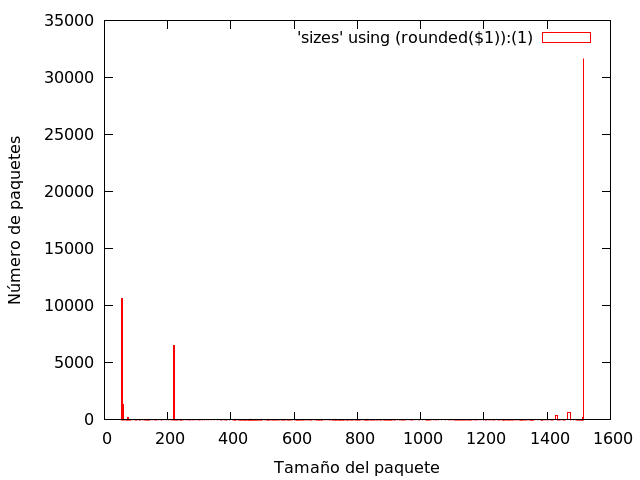
\includegraphics[width=0.8\textwidth]{imgs/Memoria/mem_sizes.png}
	\end{center}

	\item \textbf{hist\_arrivals.gp} Genera un histograma (en imgs/arrivals.png) a partir del fichero arrivals.dat (que contiene los tiempos de llegadas entre cada paquete que pase el filtro). El ancho del histograma es de 0.05 segundos.

	Para generar este ejemplo se han utilizado los puertos 

	\begin{itemize}
		\item origen: 80
		\item destino:55865
	\end{itemize}
	y descartado los pocos paquetes que han tardado más de 1.5 segundos en llegar para ejemplificar mejor el histograma generado por este fichero.
	\begin{center}
	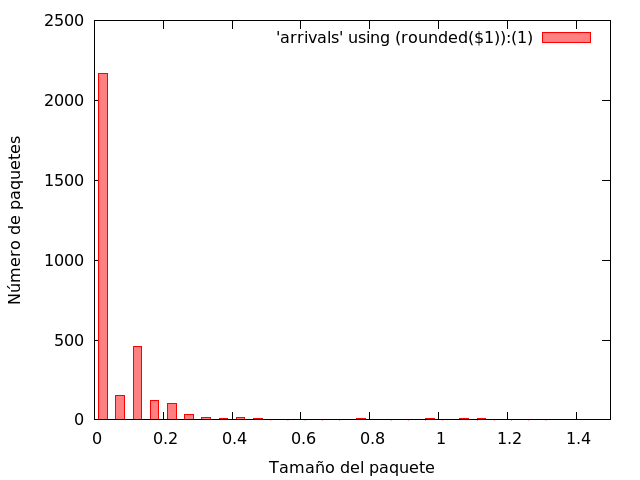
\includegraphics[width=0.8\textwidth]{imgs/Memoria/mem_arrivals_port.png}
	\end{center}
\end{itemize}

\section{Gr\'aficas pedidas}
\subsection{Ejercicio 4}

El tiempo entre paquetes entre los puertos origen: 24704 y destino:27088 presenta el siguiente histograma (generado con el script hist\_arrivals.gp)

	\begin{center}
	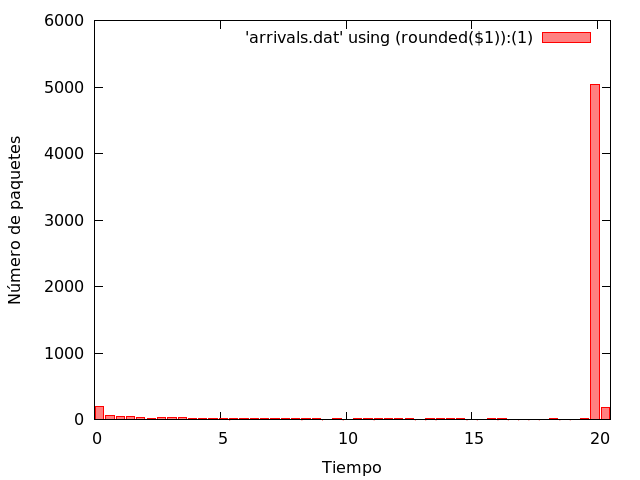
\includegraphics[width=0.8\textwidth]{imgs/Memoria/mem_arrivals_5.png}
	\end{center}

Lo cual sugiere que la comunicación entre estos equipos es muy constante ya que casi todos los paquetes se transmiten equiespaciados de tiempo (aunque no tiene mucho ancho de banda)

\subsubsection{Ejercicio 5}

El caudal/throughput/tasa/ancho de banda tomando como dirección ethernet origen \\00:55:22:af:c6:37 presenta el siguiente histograma:

\begin{center}
	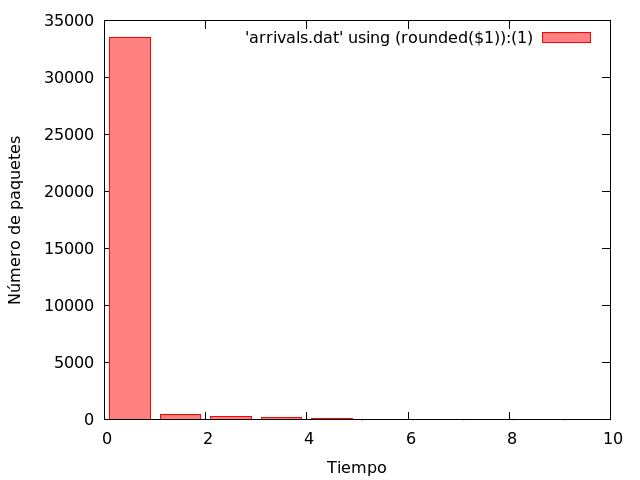
\includegraphics[width=0.8\textwidth]{imgs/Memoria/mem_caudal.png}
\end{center}

Y podemos observar que en este caso, practicamente todos los paquetes se han transmitido en el primer segundo, consumiendo un gran ancho de banda.

\end{document}